\section{3. Runtime and Protocol
Implementation}\label{runtime-and-protocol-implementation}

This section shows where MCP-Geo actually runs and how requests are
mediated, guarded, and returned.

\subsection{3.1 HTTP server, config, and
guardrails}\label{http-server-config-and-guardrails}

This subsection covers the FastAPI entrypoint, the main operational
middleware, and the config surface that controls behavior.

The repo's HTTP runtime starts in
\href{https://github.com/chris-page-gov/mcp-geo/blob/fe862910da246ca77f374cfbe484985f5df4d316/server/main.py\#L19-L216}{server/main.py},
where FastAPI routers, rate limiting, observability, and error handling
are wired together, while
\href{https://github.com/chris-page-gov/mcp-geo/blob/fe862910da246ca77f374cfbe484985f5df4d316/server/config.py}{server/config.py},
\href{https://github.com/chris-page-gov/mcp-geo/blob/fe862910da246ca77f374cfbe484985f5df4d316/server/security.py}{server/security.py},
\href{https://github.com/chris-page-gov/mcp-geo/blob/fe862910da246ca77f374cfbe484985f5df4d316/server/logging.py}{server/logging.py},
and
\href{https://github.com/chris-page-gov/mcp-geo/blob/fe862910da246ca77f374cfbe484985f5df4d316/server/observability.py}{server/observability.py}
explain how configuration, redaction, and metrics are handled. Open this
cluster when the question is about runtime behavior rather than domain
content.

Where to go:
\href{https://github.com/chris-page-gov/mcp-geo/blob/fe862910da246ca77f374cfbe484985f5df4d316/server/main.py\#L1-L216}{server/main.py},
\href{https://github.com/chris-page-gov/mcp-geo/blob/fe862910da246ca77f374cfbe484985f5df4d316/server/config.py}{server/config.py},
\href{https://github.com/chris-page-gov/mcp-geo/blob/fe862910da246ca77f374cfbe484985f5df4d316/server/security.py}{server/security.py},
\href{https://github.com/chris-page-gov/mcp-geo/blob/fe862910da246ca77f374cfbe484985f5df4d316/server/logging.py}{server/logging.py},
and
\href{https://github.com/chris-page-gov/mcp-geo/blob/fe862910da246ca77f374cfbe484985f5df4d316/server/observability.py}{server/observability.py}.

\subsection{3.2 STDIO transport and MCP protocol
machinery}\label{stdio-transport-and-mcp-protocol-machinery}

This subsection points to the files that make MCP-Geo interoperable with
clients that speak JSON-RPC over STDIO or HTTP.

The transport and protocol layer is concentrated in
\href{https://github.com/chris-page-gov/mcp-geo/blob/fe862910da246ca77f374cfbe484985f5df4d316/server/stdio_adapter.py\#L1-L260}{server/stdio\_adapter.py},
\href{https://github.com/chris-page-gov/mcp-geo/blob/fe862910da246ca77f374cfbe484985f5df4d316/server/protocol.py}{server/protocol.py},
and the
\href{https://github.com/chris-page-gov/mcp-geo/tree/fe862910da246ca77f374cfbe484985f5df4d316/server/mcp}{server/mcp/}
package, which holds
\href{https://github.com/chris-page-gov/mcp-geo/blob/fe862910da246ca77f374cfbe484985f5df4d316/server/mcp/http_transport.py}{HTTP
transport},
\href{https://github.com/chris-page-gov/mcp-geo/blob/fe862910da246ca77f374cfbe484985f5df4d316/server/mcp/resources.py}{resource
handling},
\href{https://github.com/chris-page-gov/mcp-geo/blob/fe862910da246ca77f374cfbe484985f5df4d316/server/mcp/tool_search.py}{tool
search},
\href{https://github.com/chris-page-gov/mcp-geo/blob/fe862910da246ca77f374cfbe484985f5df4d316/server/mcp/prompts.py}{prompts},
and
\href{https://github.com/chris-page-gov/mcp-geo/blob/fe862910da246ca77f374cfbe484985f5df4d316/server/mcp/elicitation_forms.py}{elicitation
forms}. This is the place to look when client behavior, protocol
negotiation, or tool-discovery shape is the issue.

Where to go:
\href{https://github.com/chris-page-gov/mcp-geo/blob/fe862910da246ca77f374cfbe484985f5df4d316/server/stdio_adapter.py\#L1-L260}{server/stdio\_adapter.py},
\href{https://github.com/chris-page-gov/mcp-geo/blob/fe862910da246ca77f374cfbe484985f5df4d316/server/protocol.py}{server/protocol.py},
\href{https://github.com/chris-page-gov/mcp-geo/blob/fe862910da246ca77f374cfbe484985f5df4d316/server/mcp/http_transport.py}{server/mcp/http\_transport.py},
\href{https://github.com/chris-page-gov/mcp-geo/blob/fe862910da246ca77f374cfbe484985f5df4d316/server/mcp/resources.py}{server/mcp/resources.py},
\href{https://github.com/chris-page-gov/mcp-geo/blob/fe862910da246ca77f374cfbe484985f5df4d316/server/mcp/tool_search.py}{server/mcp/tool\_search.py},
and
\href{https://github.com/chris-page-gov/mcp-geo/blob/fe862910da246ca77f374cfbe484985f5df4d316/server/mcp/elicitation_forms.py}{server/mcp/elicitation\_forms.py}.

\begin{figure}
\centering
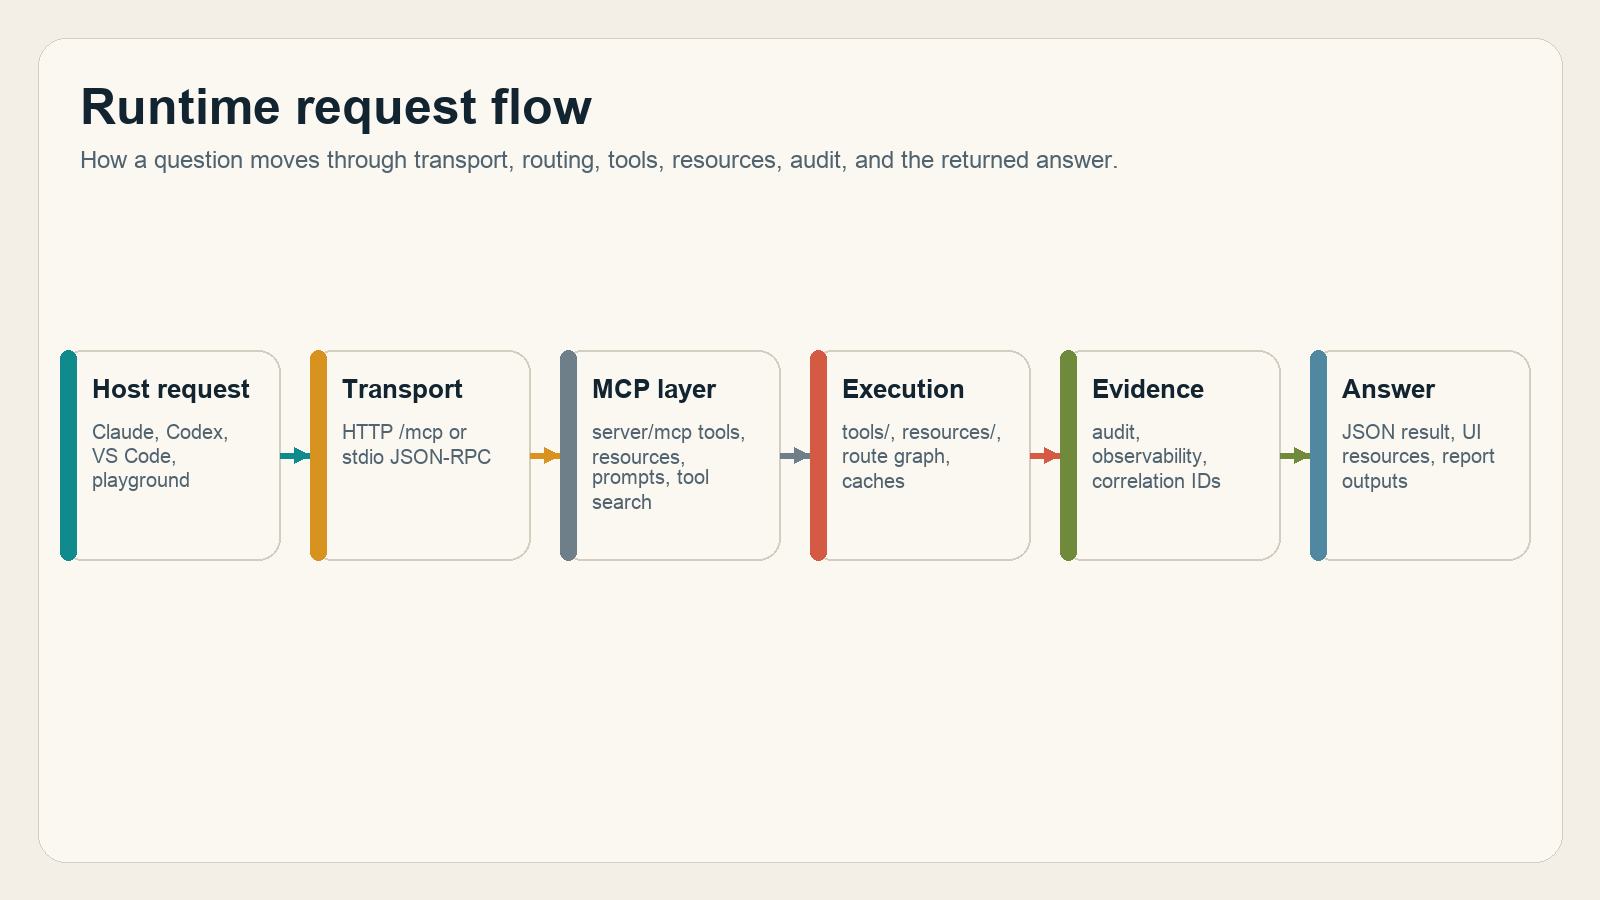
\includegraphics[width=0.96\linewidth,height=\textheight,keepaspectratio,alt={Figure F03. Runtime request flow}]{figures/f03_runtime_request_flow.png}
\caption{Figure F03. Runtime request flow}
\end{figure}

Figure F03 turns the transport story into a single governed path from
host request to audited response.

\subsection{3.3 Audit, cache, and route-planning
subsystems}\label{audit-cache-and-route-planning-subsystems}

This subsection groups the supporting subsystems that turn the server
from a thin transport wrapper into a governed answer engine.

Three deeper runtime areas matter here. The
\href{https://github.com/chris-page-gov/mcp-geo/tree/fe862910da246ca77f374cfbe484985f5df4d316/server/audit}{audit
subsystem} packages decision records, redaction, disclosure, integrity,
and source registers; the cache layer lives in
\href{https://github.com/chris-page-gov/mcp-geo/blob/fe862910da246ca77f374cfbe484985f5df4d316/server/boundary_cache.py}{server/boundary\_cache.py},
\href{https://github.com/chris-page-gov/mcp-geo/blob/fe862910da246ca77f374cfbe484985f5df4d316/server/ons_geo_cache.py}{server/ons\_geo\_cache.py},
and
\href{https://github.com/chris-page-gov/mcp-geo/blob/fe862910da246ca77f374cfbe484985f5df4d316/server/dataset_cache.py}{server/dataset\_cache.py};
and route-planning logic is concentrated in
\href{https://github.com/chris-page-gov/mcp-geo/blob/fe862910da246ca77f374cfbe484985f5df4d316/server/route_graph.py}{server/route\_graph.py}
and
\href{https://github.com/chris-page-gov/mcp-geo/blob/fe862910da246ca77f374cfbe484985f5df4d316/server/route_planning.py}{server/route\_planning.py}.
These are the files that explain why the repo is about evidence
discipline as well as tool exposure.

Where to go:
\href{https://github.com/chris-page-gov/mcp-geo/tree/fe862910da246ca77f374cfbe484985f5df4d316/server/audit}{server/audit/},
\href{https://github.com/chris-page-gov/mcp-geo/blob/fe862910da246ca77f374cfbe484985f5df4d316/server/boundary_cache.py}{server/boundary\_cache.py},
\href{https://github.com/chris-page-gov/mcp-geo/blob/fe862910da246ca77f374cfbe484985f5df4d316/server/ons_geo_cache.py}{server/ons\_geo\_cache.py},
\href{https://github.com/chris-page-gov/mcp-geo/blob/fe862910da246ca77f374cfbe484985f5df4d316/server/dataset_cache.py}{server/dataset\_cache.py},
\href{https://github.com/chris-page-gov/mcp-geo/blob/fe862910da246ca77f374cfbe484985f5df4d316/server/route_graph.py}{server/route\_graph.py},
and
\href{https://github.com/chris-page-gov/mcp-geo/blob/fe862910da246ca77f374cfbe484985f5df4d316/server/route_planning.py}{server/route\_planning.py}.
